\documentclass[slidestop]{beamer}
\usepackage{beamerthemesplit}
\usepackage{graphics,epsfig}
\usepackage{pstricks}
\usepackage{graphicx}
\usepackage{hyperref}
\usepackage{subfigure}
\usepackage{listings}
\usepackage{multirow}
\usepackage{xspace}
\usepackage[absolute,overlay]{textpos}
\usepackage{tikz}
\usetikzlibrary{decorations}
\usetikzlibrary{decorations.pathmorphing}
\usetikzlibrary{shapes,arrows}
\setlength{\TPHorizModule}{1cm}
\setlength{\TPVertModule}{1cm}


\mode<presentation>
{ \usetheme{Boadilla}
  \setbeamercovered{transparent}
  \setbeamertemplate{items}[circle]
  \setbeamertemplate{theorems}[numbered]
  \setbeamertemplate{footline}[frame number]
}
 
%\useinnertheme[shadow=true]{rounded}
\useoutertheme{shadow}
\usecolortheme{whale}

\newcommand\blfootnote[1]{
  \begingroup
  \renewcommand\thefootnote{}\footnote{#1}
  \addtocounter{footnote}{-1}
  \endgroup
}

\mode
<all>

\title{C Programming}
\author{Wan-Lei Zhao}

\makeatletter

\begin{document}
\begin{frame}
   \begin{center}
    \vspace{24pt}
    \Huge\textbf{C Programming}\blfootnote{Email: wlzhao@xmu.edu.cn, copyrights are fully reserved by the author.}\\
     \Huge{Lecture 11: make \& Makefile}
     \begin{figure}
\begin{center}
	
\includegraphics[width=0.3\linewidth]{figs/makelogo.pdf}
\end{center}
\end{figure}
    \vspace{23pt}
  \end{center}
  \begin{align*}
   \vspace{18pt}
      \large{\mbox{Lecturer:}~Dr.~\mbox{Wan-Lei~~Zhao}} \\
      \large{Autumn~~Semester~~2022} \\
   \vspace{30pt}
  \end{align*}
\end{frame}

\definecolor{cornblue}{HTML}{6495ED}
\definecolor{navyblue}{HTML}{000080}
\definecolor{midnblue}{HTML}{191970}
\definecolor{lghtblue}{HTML}{B0C4DE}
\setbeamercolor{background}{fg=black, bg=lghtblue}
\setbeamercolor{palette primary}{fg=white, bg=lghtblue}
\setbeamercolor{palette secondary}{fg=black, bg=cornblue}
\setbeamercolor{palette tertiary}{fg=black, bg=lghtblue}
\setbeamercolor{palette quaternary}{fg=black, bg=lghtblue}
\setbeamercolor{frametitle}{fg=black, bg=white}
\definecolor{ballblue}{rgb}{0.13, 0.67, 0.8}
\definecolor{cornflowerblue}{rgb}{0.39,0.58,0.93}
\definecolor{babyblueeyes}{rgb}{0.63, 0.79, 0.95}

\setbeamertemplate{footline}
{
  \leavevmode%
  \hbox{%
  \begin{beamercolorbox}[wd=.275\paperwidth,ht=2.25ex,dp=1ex,center]{author in head/foot}%
    \usebeamerfont{author in head/foot}\insertshortauthor
  \end{beamercolorbox}%
  \begin{beamercolorbox}[wd=.44\paperwidth,ht=2.25ex,dp=1ex,center]{title in head/foot}%
    \usebeamerfont{title in head/foot}\insertshorttitle\hspace*{3em}
    \hspace*{1ex}
  \end{beamercolorbox}%
  \begin{beamercolorbox}[wd=.285\paperwidth,ht=2.25ex,dp=1ex,center]{date/foot}%
    \usebeamerfont{title in head/foot}\hspace*{2em}
    \insertframenumber{} / \inserttotalframenumber\hspace*{1ex}
  \end{beamercolorbox}}%
  \vskip0pt
}



% preset-listing options
\lstset{
  backgroundcolor=\color{white},   
  basicstyle=\footnotesize,    
  language=c,
  breakatwhitespace=false,         
  breaklines=true,                 % sets automatic line breaking
  captionpos=b,                    % sets the caption-position to bottom
  commentstyle=\color{ballblue},    % comment style
  extendedchars=true,              
  frame=single,                    % adds a frame around the code     
  keywordstyle=\color{blue},       % keyword style
  numbers=left,                    
  numbersep=5pt,                   
  numberstyle=\tiny\color{blue}, 
  rulecolor=\color{babyblueeyes},
  stepnumber=1,              
  stringstyle=\color{black},     % string literal style
  tabsize=4,                       % sets default tabsize to 4 spaces
  title=\lstname                   
}


\section{Build Project with Make}
\label{sec:make}
\begin{frame}<beamer>
    \frametitle{Outline}
    \tableofcontents[currentsection]
\end{frame}

\begin{frame}[fragile]{Why make? (1)}
\vspace{-0.3in}
\begin{columns}
\begin{column}{0.4\linewidth}
\begin{lstlisting}{mylib.h}}[linewidth=0.9\linewidth]
#ifndef MYLIB_H
#define MYLIB_H
int isodd(int x);
float square(float x);
#endif
\end{lstlisting}
\vspace{-0.1in}
\begin{lstlisting}{mylib.c}[linewidth=0.9\linewidth]
#include "mylib.h"
float square(float x){
    return x*x;
}

int isodd(int x){
    if(x%2 != 0)
      return 1;
    else
      return 0;
}
\end{lstlisting}
\end{column}
\begin{column}{0.54\linewidth}
\begin{lstlisting}{main.c}
#include "mylib.h"
#include <stdio.h>
int main(){
  float x = 3.4;
  int a = 5;
  float y = square(x);
  if(isodd(a))
  {
       printf("%d is odd\n", a);
  }
  return 0;
}
\end{lstlisting}
\vspace{-0.15in}
\begin{lstlisting}{Build the project}[language=make]
gcc myproj.c -o myproj.o -c
gcc mylib.c -o mylib.o -c

gcc -o myproj myproj.o mylib.o
\end{lstlisting}
\end{column}
\end{columns}
\end{frame}

\begin{frame}[fragile]{Why make? (2)}

\begin{lstlisting}[language=make, linewidth=0.75\linewidth, firstnumber=1,caption="Build the project"]
gcc myproj.c -o myproj.o -c
gcc mylib.c -o mylib.o -c

gcc -o myproj myproj.o mylib.o
\end{lstlisting}
\begin{itemize}
	\item {In practice, we may have many libraries to compile and link}
	\vspace{0.15in}
	\item {\textcolor{red}{gcc} -o \textcolor{green}{myproj} myproj.o mylib.o}
	\vspace{0.15in}
	\item {If we do it manually, it is too laborious!!!}
\end{itemize}

\begin{itemize}
	\item {This is where ``Makefile'' comes to fit in}
\end{itemize}
\end{frame}

\begin{frame}{Makefile}
\begin{itemize}
	\item {A script file organize all the compilation things together}
		\vspace{0.15in}
	\item {It is responsible for}
		\vspace{0.15in}
		\begin{enumerate}
			\item {Compiling the source files (compile from \textcolor{red}{.c} to  \textcolor{red}{.o})}
			\vspace{0.15in}
			\item {Linking the files into the final executable software}
			\vspace{0.15in}
			\item {Installing the software to target directory}
		\end{enumerate}
		\item {Command \textcolor{red}{make} will parse the script}
		\item {It fulfills the intructions in the script}
\end{itemize}
\end{frame}

\begin{frame}[fragile]{Prepare Environment (1)}
\begin{itemize}
	\item {Define the variables}
\end{itemize}
\lstset{language=[gnu] make}
\lstset{
   language=[gnu] make,
   keywordstyle=\color{teal}\textbf,
   stringstyle=\color{blue},
   identifierstyle=\itshape
}
\begin{lstlisting}[linewidth=0.9\linewidth, xleftmargin=0.05\linewidth]
WORK_DIR=.
CC=gcc
LD=gcc
OBJ_DIR=$(WORK_DIR)/obj
OBJ_RELEASE=$(OBJ_DIR)/mylib.o $(OBJ_DIR)/myproj.o
RELEASE=$(WORK_DIR)/bin/myproj
\end{lstlisting}

\begin{itemize}
	\item {command \textcolor{red}{make} supports environment variable definitions }
\end{itemize}
\begin{center}
	\Large{VARIABLE\_NAME = value}
\end{center}
\begin{itemize}
	\item {One can specify the file, directory, command, compilation parameters}
	\item {They may support the compilation of the project}
\end{itemize}
\end{frame}


\begin{frame}[fragile]{Prepare Environment (2)}
\lstset{
   language=[gnu] make,
   keywordstyle=\color{teal}\textbf,
   stringstyle=\color{blue},
   identifierstyle=\itshape
}
\begin{lstlisting}[linewidth=0.9\linewidth, xleftmargin=0.05\linewidth]{Makefile}
WORK_DIR=.
CC=gcc
LD=gcc
\end{lstlisting}
\vspace{-0.2in}
\begin{itemize}
	\item {Command \textcolor{red}{make} supports environment variable definitions }
\end{itemize}
\begin{center}
	\Large{WORK\_DIR = .}
\end{center}
\begin{itemize}
	\item {Specify the project directory where ``Makefile'' and the project is located}
	\item {The  variable name is by convention \textcolor{red}{CAPITALIZED}}
\end{itemize}
\end{frame}

\begin{frame}[fragile]{Prepare Environment (3)}
\lstset{language=[gnu] make}
\lstset{
   language=[gnu] make,
   keywordstyle=\color{teal}\textbf,
   stringstyle=\color{blue},
   identifierstyle=\itshape
}
\begin{lstlisting}[linewidth=0.9\linewidth, xleftmargin=0.05\linewidth, caption=Makefile]
WORK_DIR=.
CC=gcc
LD=gcc
\end{lstlisting}
\vspace{-0.2in}
\begin{itemize}
	\item {Command \textcolor{red}{make} supports environment variable definitions }
\end{itemize}
\begin{center}
	\Large{CC=gcc}\\
	\Large{LD=gcc}
\end{center}
\begin{itemize}
	\item {``CC=gcc'' specifies the compiler}
	\item {``LD=gcc'' specifies the linker}
\end{itemize}
\end{frame}

\begin{frame}[fragile]{Prepare Environment (4)}
\vspace{-0.2in}
\lstset{language=[gnu] make}
\lstset{
   language=[gnu] make,
   keywordstyle=\color{teal}\textbf,
   stringstyle=\color{blue},
   identifierstyle=\itshape
}
\begin{lstlisting}[linewidth=0.9\linewidth, xleftmargin=0.05\linewidth, caption=Makefile]
OBJ_DIR=$(WORK_DIR)/obj
OBJ_RELEASE=$(OBJ_DIR)/mylib.o $(OBJ_DIR)/myproj.o
RELEASE=$(WORK_DIR)/bin/myproj
\end{lstlisting}
\vspace{-0.2in}
\begin{itemize}
	\item {Command \textcolor{red}{make} supports environment variable definitions }
\end{itemize}
\begin{center}
	\Large{\$(WORK\_DIR)/obj}
\end{center}
\vspace{-0.2in}
\begin{itemize}
	\item {\$(VARIABLE) cite the value of the VARIABLE}
	\item {Here ``\$(WORK\_DIR)'' is replaced by ``./''}
\end{itemize}
\end{frame}


\begin{frame}[fragile]{Prepare Environment (5)}
\vspace{-0.2in}
\lstset{language=[gnu] make}
\lstset{
   language=[gnu] make,
   keywordstyle=\color{teal}\textbf,
   stringstyle=\color{blue},
   identifierstyle=\itshape
}
\begin{lstlisting}[linewidth=0.9\linewidth, xleftmargin=0.05\linewidth, caption=Makefile]
OBJ_DIR=$(WORK_DIR)/obj
OBJ_RELEASE=$(OBJ_DIR)/mylib.o $(OBJ_DIR)/myproj.o
RELEASE=$(WORK_DIR)/bin/myproj
\end{lstlisting}
\vspace{-0.1in}
\begin{itemize}
	\item {The above instructions indicate}
	\begin{enumerate}
		\item {The object files will be put to \textcolor{red}{./obj/}}
		\item {``OBJ\_RELEASE'' keeps the lists of all object files}
		\item {The final target binary software name is ``myproj''}
		\item {It will be put to \textcolor{red}{./bin/}}
	\end{enumerate}
\end{itemize}

\end{frame}


\begin{frame}[fragile]{Prepare Environment (6)}
\lstset{language=[gnu] make}
\lstset{
   language=[gnu] make,
   keywordstyle=\color{teal}\textbf,
   stringstyle=\color{blue},
   identifierstyle=\itshape
}
\begin{lstlisting}[linewidth=0.9\linewidth, xleftmargin=0.05\linewidth]
WORK_DIR=.
CC=gcc
LD=gcc
OBJ_DIR=$(WORK_DIR)/obj
OBJ_RELEASE=$(OBJ_DIR)/mylib.o $(OBJ_DIR)/myproj.o
RELEASE=$(WORK_DIR)/bin/myproj
\end{lstlisting}

\begin{enumerate}
	\item {We know the working directory }
	\item {We have the compiler and linker}
	\item {We know where we should put the object files}
	\item {We know where we should put the target binary file}
\end{enumerate}
\end{frame}

\begin{frame}[fragile]{Prepare Environment (7)}
\lstset{language=[gnu] make}
\lstset{
   language=[gnu] make,
   keywordstyle=\color{teal}\textbf,
   stringstyle=\color{blue},
   identifierstyle=\itshape
}
\begin{lstlisting}[linewidth=0.9\linewidth, xleftmargin=0.05\linewidth]
WORK_DIR=.
CC=gcc
LD=gcc
OBJ_DIR=$(WORK_DIR)/obj
OBJ_RELEASE=$(OBJ_DIR)/mylib.o $(OBJ_DIR)/myproj.o
RELEASE=$(WORK_DIR)/bin/myproj

before_release:
        test -d bin || mkdir -p bin
        test -d $(OBJ_DIR) || mkdir -p $(OBJ_DIR)
\end{lstlisting}

\begin{enumerate}
	\item {However, ``./obj/'' and ``./bin/'' are not ready }
	\item {We can test and make them if necessary}
\end{enumerate}
\end{frame}

\begin{frame}[fragile]{Compile the source file}
\lstset{language=[gnu] make}
\lstset{
   language=[gnu] make,
   keywordstyle=\color{teal}\textbf,
   stringstyle=\color{blue},
   identifierstyle=\itshape
}
\begin{lstlisting}[linewidth=0.9\linewidth, xleftmargin=0.05\linewidth]
$(OBJ_DIR)/mylib.o: mylib.c
        $(CC) -c mylib.c -o $(OBJ_DIR)/mylib.o
\end{lstlisting}
\vspace{-0.15in}
\begin{itemize}
	\item {Instruction ``\$(OBJ\_DIR)/mylib.o'' compiles ``mylib.c''}
	\item {The compilation relies on file ``mylib.c''}
	\item {The indentation should  be by ``Tab''}
	\item {We can do so for all the source files}
	\item {The resulting file is put to ``./obj/mylib.o'' }
\end{itemize}
\begin{lstlisting}[linewidth=0.9\linewidth, xleftmargin=0.05\linewidth]
$(OBJ_DIR)/mylib.o: mylib.c
        $(CC) -c mylib.c -o $(OBJ_DIR)/mylib.o
        
$(OBJ_DIR)/myproj.o: myproj.c
        $(CC) -c myproj.c -o $(OBJ_DIR)/myproj.o
\end{lstlisting}
\end{frame}

\begin{frame}[fragile]{Link the source file}
\lstset{language=[gnu] make}
\lstset{
   language=[gnu] make,
   keywordstyle=\color{teal}\textbf,
   stringstyle=\color{blue},
   identifierstyle=\itshape
}
\begin{lstlisting}[linewidth=0.9\linewidth, xleftmargin=0.05\linewidth]
release: $(OBJ_RELEASE)
        $(LD) -o $(RELEASE) $(OBJ_RELEASE)
\end{lstlisting}
\vspace{-0.15in}
\begin{itemize}
	\item {The project will be linked with mylib.o and myproj.o}
	\item {The list of object files are kept in ``\$(OBJ\_RELEASE)''}
	\item {\$(LD) calls ``gcc''}
	\item {The target is specified by ``\$(RELEASE)''}
\end{itemize}

\end{frame}

\begin{frame}[fragile]{Build the whole project}
\lstset{language=[gnu] make}
\lstset{
   language=[gnu] make,
   keywordstyle=\color{teal}\textbf,
   stringstyle=\color{blue},
   identifierstyle=\itshape
}
\begin{lstlisting}[linewidth=0.9\linewidth, xleftmargin=0.05\linewidth]
release: before_release $(OBJ_RELEASE)
        $(LD) -o $(RELEASE) $(OBJ_RELEASE)
\end{lstlisting}
\vspace{-0.15in}
\begin{itemize}
	\item {The instruction ``release''  relies on another two intructions}
	\item {``before\_release'' and ``\$(OBJ\_RELEASE)''}
	\item {``\$(OBJ\_RELEASE)'' are a list of instructions}
	\begin{enumerate}
		\item {Run instruction ``before\_release''}
		\item {Run list of instructions in ``\$(OBJ\_RELEASE)''}
		\item {Run \$(LD) -o \$(RELEASE) \$(OBJ\_RELEASE)}
	\end{enumerate}
\end{itemize}

\end{frame}


\begin{frame}[fragile]{Clean the object files}
\lstset{language=[gnu] make}
\lstset{
   language=[gnu] make,
   keywordstyle=\color{teal}\textbf,
   stringstyle=\color{blue},
   identifierstyle=\itshape
}
\begin{itemize}
	\item {In some cases, we may want to clean the object files}
\end{itemize}
\begin{lstlisting}[linewidth=0.9\linewidth, xleftmargin=0.05\linewidth]
clean:
        rm -rf $(OBJ_DIR)/*.o
        rm -rf $(RELEASE)
\end{lstlisting}
\vspace{-0.15in}
\begin{itemize}
	\item {We call command ``rm''}
	\item {We label the instruction as ``clean''}
\end{itemize}

\end{frame}

\begin{frame}[fragile]{A Complete Makefile}
\vspace{-0.2in}
\lstset{language=[gnu] make}
\lstset{
   language=[gnu] make,
   keywordstyle=\color{teal}\textbf,
   stringstyle=\color{blue},
   identifierstyle=\itshape
}
\begin{lstlisting}[linewidth=0.9\linewidth, xleftmargin=0.05\linewidth]{Makefile}
WORK_DIR=.
CC=gcc
LD=gcc
OBJ_DIR=$(WORK_DIR)/obj
OBJ_RELEASE=$(OBJ_DIR)/mylib.o $(OBJ_DIR)/myproj.o
RELEASE=$(WORK_DIR)/bin/myproj

$(OBJ_DIR)/mylib.o: mylib.c
        $(CC) -c mylib.c -o $(OBJ_DIR)/mylib.o

$(OBJ_DIR)/myproj.o: myproj.c
        $(CC) -c myproj.c -o $(OBJ_DIR)/myproj.o

before_release:
        test -d bin || mkdir -p bin
        test -d $(OBJ_DIR) || mkdir -p $(OBJ_DIR)

release: before_release $(OBJ_RELEASE)
        $(LD) -o $(RELEASE) $(OBJ_RELEASE)
\end{lstlisting}

\end{frame}

\begin{frame}[fragile]{A Complete Makefile}

\begin{lstlisting}[linewidth=0.9\linewidth, xleftmargin=0.05\linewidth]{Makefile}
clean:
        rm -rf $(OBJ_DIR)/*.o
        rm -rf $(RELEASE)
\end{lstlisting}
\begin{itemize}
	\item {Five major sections}
	\begin{enumerate}
		\item {Define the environment variables}
		\item {Prepare directories}
		\item {Instructions of compiling source files to object files}
		\item {Link object files to target binary executable or library}
		\item {Instructions to clean the object files}
	\end{enumerate}
\end{itemize}
\end{frame}


\begin{frame}{Running Flow inside Makefile (1)}
\begin{figure}
	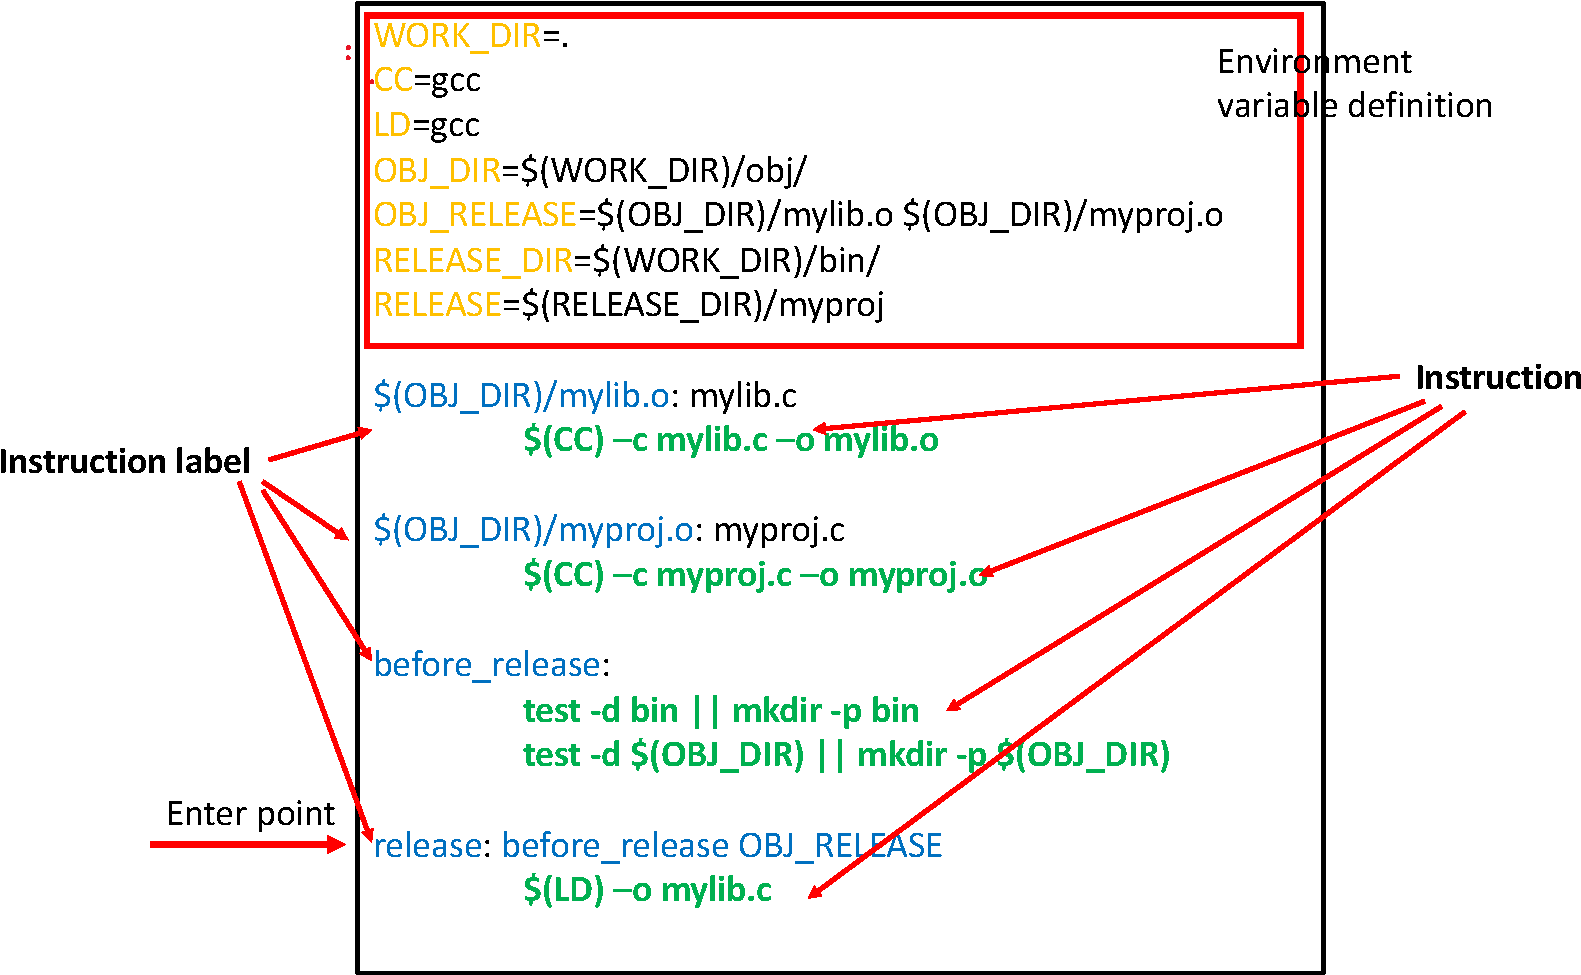
\includegraphics[width=0.80\linewidth]{figs/make1.pdf}
\end{figure}
\begin{itemize}
	\item {Run command ``\textcolor{blue}{make release}''}
\end{itemize}
\end{frame}

\begin{frame}{Running Flow inside Makefile (2)}
\begin{figure}
	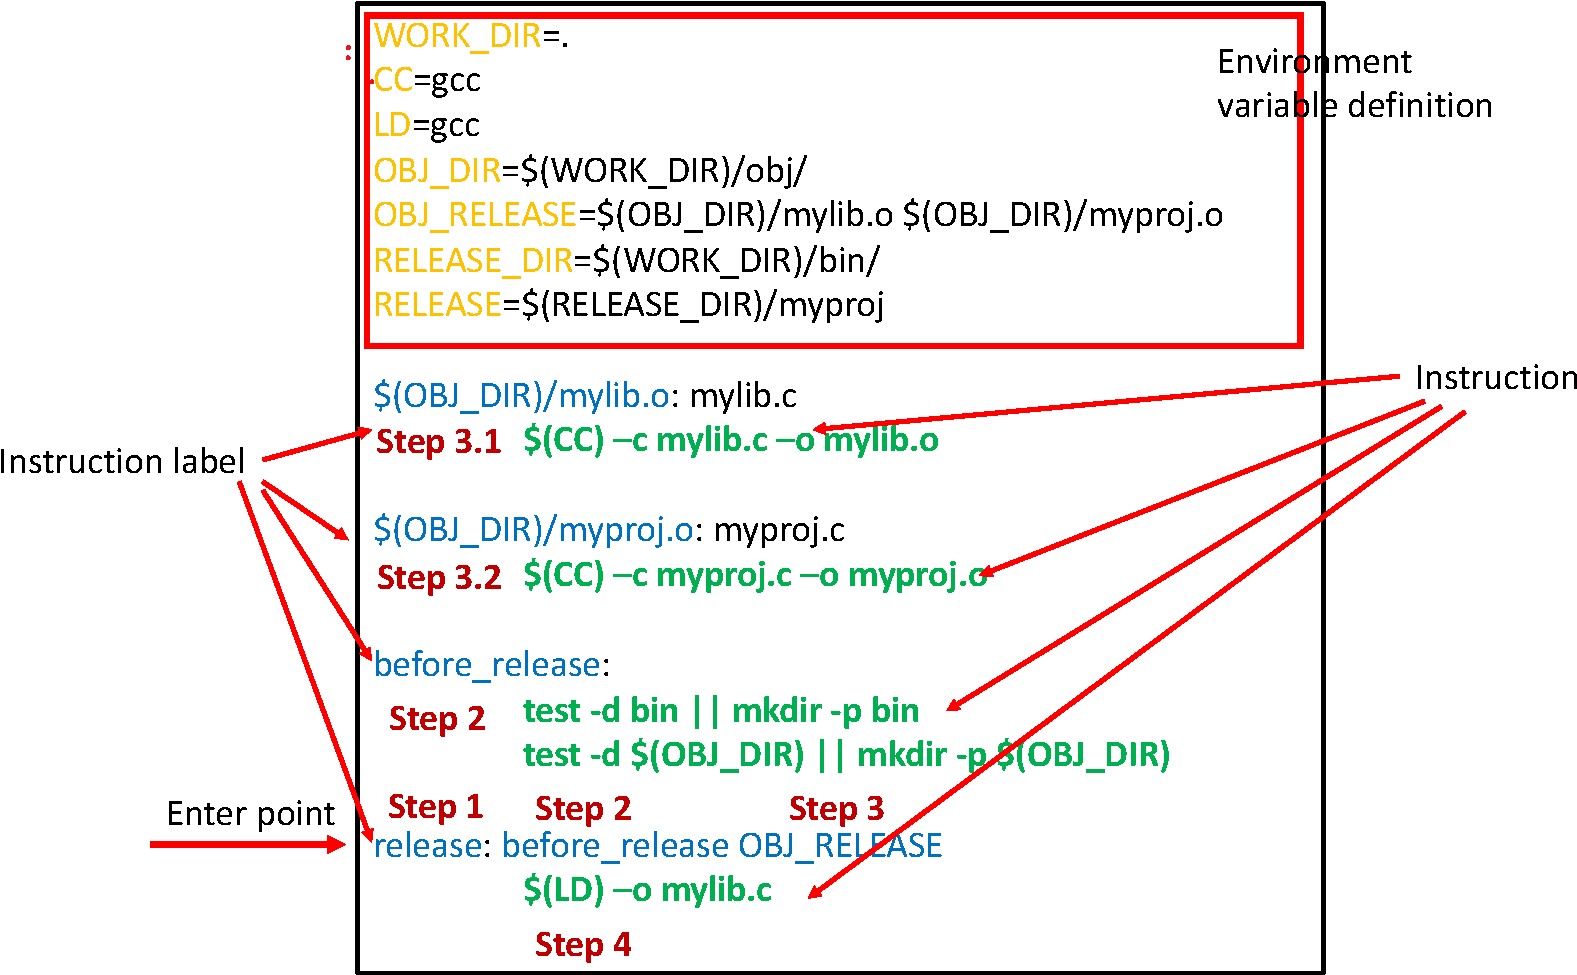
\includegraphics[width=0.80\linewidth]{figs/make2.pdf}
\end{figure}
\begin{itemize}
	\item {Run command ``\textcolor{blue}{make release}''}
\end{itemize}
\end{frame}

\begin{frame}[fragile]{Add libraries in Makefile (1)}
\begin{itemize}
	\item {We may need either static or dynamic libraries or both}
\end{itemize}
\begin{lstlisting}[linewidth=0.9\linewidth, firstnumber=1, xleftmargin=0.05\linewidth]{myproj.c}
#include <math.h>
#include "mylib.h"
#include <stdio.h>
int main(){
  float x = 3.4;
  int a = 5;
  float y = square(x);
  float z = sqrt(x);
  return 0;
}
\end{lstlisting}
\begin{itemize}
	\item {For this code, we should compile it by}
\end{itemize}
\begin{lstlisting}[linewidth=0.9\linewidth, xleftmargin=0.05\linewidth]
gcc -o myproj myproj.o mylib.o -lm
\end{lstlisting}
\end{frame}

\begin{frame}[fragile]{Add libraries in Makefile (2)}
\vspace{-0.2in}
\begin{lstlisting}[linewidth=0.95\linewidth, firstnumber= 1, xleftmargin=0.02\linewidth]{Makefile}
WORK_DIR=.
CC=gcc
LD=gcc
LDFLAGS= -lm
OBJ_DIR=$(WORK_DIR)/obj
OBJ_RELEASE=$(OBJ_DIR)/mylib.o $(OBJ_DIR)/myproj.o
RELEASE=$(WORK_DIR)/bin/myproj

$(OBJ_DIR)/mylib.o: mylib.c
        $(CC) -c mylib.c -o $(OBJ_DIR)/mylib.o

$(OBJ_DIR)/myproj.o: myproj.c
        $(CC) -c myproj.c -o $(OBJ_DIR)/myproj.o

before_release:
        test -d bin || mkdir -p bin
        test -d $(OBJ_DIR) || mkdir -p $(OBJ_DIR)

release: before_release $(OBJ_RELEASE)
        $(LD) $(LDFLAGS) -o $(RELEASE) $(OBJ_RELEASE)
\end{lstlisting}

\end{frame}

\section{Build Project with CMake}
\label{sec:cmake}
\begin{frame}<beamer>
    \frametitle{Outline}
    \tableofcontents[currentsection]
\end{frame}

\begin{frame}{Why cmake?}
\vspace{0.3in}
\begin{itemize}
	\item {However, writing a Makefile line-by-line is still too sweaty}
	\item {There are several convenient ways}
	\begin{enumerate}
			\item {``cbp2make''\footnote{https://sourceforge.net/projects/cbp2make/}}
			\begin{itemize}
				\item {It works with CodeBlocks}
					\vspace{0.15in}
				\item {Command: cbp2make -in project.cbp -out Makefile}
			\end{itemize}
				\vspace{0.15in}
			\item {cmake\footnote{https://cmake.org/}}
			\begin{itemize}
				\item {It is a powerful cross-platform tool for C/C++ project compilation, test, and installation}
					\vspace{0.15in}
				\item {Based on a ``CMakeLists.txt'' input file, it produces ``Makefile''}
			\end{itemize}
	\end{enumerate}
\end{itemize}

\end{frame}

\begin{frame}{About cmake}
\vspace{0.2in}
\begin{figure}
	\begin{center}
		
\includegraphics[width=0.3\linewidth]{figs/cmake.png}
	\end{center}
\end{figure}
\begin{itemize}
	\item {It is another useful tool}
	\vspace{0.15in}
	\item {It helps to produce the ``Makefile''}
	\vspace{0.15in}
	\item {The cmake requires another simpler script ``CMakeLists.txt''}
	\vspace{0.15in}
	\item {Compared to ``Makefile'', it is a super script and easier to compose}
\end{itemize}
\end{frame}

\begin{frame}[fragile]{Compose a ``CMakeLists.txt'' (1)}
\lstset{
   language=[gnu] make,
   keywordstyle=\color{teal}\textbf,
   stringstyle=\color{blue},
   identifierstyle=\itshape,
     basicstyle=\scriptsize,  
}
\begin{lstlisting}[linewidth=0.95\linewidth, firstnumber= 1, xleftmargin=0.02\linewidth]{CMakeLists.txt}
cmake_minimum_required (VERSION 2.8)
\end{lstlisting}

\begin{enumerate}
	\item {This cmake setting is put in \textcolor{red}{command}(\textcolor{green}{value}) pattern}
		\vspace{0.15in}
	\item {This is the way set values for environment variables \textcolor{red}{supported by cmake} }
		\vspace{0.15in}
	\item {Here we specify the minimum required cmake version is ``VERSION 2.8''}
\end{enumerate}
\end{frame}

\begin{frame}[fragile]{Compose a ``CMakeLists.txt'' (2)}
\lstset{
   language=[gnu] make,
   keywordstyle=\color{teal}\textbf,
   stringstyle=\color{blue},
   identifierstyle=\itshape,
     basicstyle=\scriptsize,  
}
\begin{lstlisting}[linewidth=0.95\linewidth, firstnumber= 1, xleftmargin=0.02\linewidth]{CMakeLists.txt}
cmake_minimum_required (VERSION 2.8)

project (proj1)
\end{lstlisting}

\begin{enumerate}
	\item {Here we specify the target project name as ``proj1''}
	\vspace{0.15in}
	\item {After compilation, the name of our executable will be ``proj1''}
\end{enumerate}
\end{frame}

\begin{frame}[fragile]{Compose a ``CMakeLists.txt'' (3)}
\lstset{
   language=[gnu] make,
   keywordstyle=\color{teal}\textbf,
   stringstyle=\color{blue},
   identifierstyle=\itshape,
     basicstyle=\scriptsize,  
}
\begin{lstlisting}[linewidth=0.95\linewidth, firstnumber= 1, xleftmargin=0.02\linewidth]{CMakeLists.txt}
cmake_minimum_required (VERSION 2.8)

project (proj1)

add_executable(proj1 myproj.c mylib.c)
\end{lstlisting}

\begin{enumerate}
	\item {``add\_executable'' allows us to list out all C/C++ source files}
	\vspace{0.15in}
	\item {The leading file name is the target file name ``proj1''}
\end{enumerate}
\end{frame}

\begin{frame}[fragile]{Compose a ``CMakeLists.txt'' (4)}
\lstset{
   language=[gnu] make,
   keywordstyle=\color{teal}\textbf,
   stringstyle=\color{blue},
   identifierstyle=\itshape,
     basicstyle=\scriptsize,  
}
\begin{lstlisting}[linewidth=0.95\linewidth, firstnumber= 1, xleftmargin=0.02\linewidth]{CMakeLists.txt}
cmake_minimum_required (VERSION 2.8)

project (proj1)

add_executable(proj1 myproj.c mylib.c)
\end{lstlisting}

\begin{enumerate}
	\item {We name this text script file as ``CMakeLists.txt''}
	\vspace{0.1in}
	\item {Put it to the same folder as the source files}
	\vspace{0.1in}
	\item {Using ``mkdir'' to make a sub folder ``build'' under the same folder}
	\vspace{0.10in}
	\item {``cd build''}
	\vspace{0.10in}
	\item {``cmake ../''}
\end{enumerate}
\begin{itemize}
	\item {After the above steps, one could see ``Makefile'' under build folder}
\end{itemize}
\end{frame}

\begin{frame}[fragile]{Compose a ``CMakeLists.txt'' (5)}
\lstset{
   language=[gnu] make,
   keywordstyle=\color{teal}\textbf,
   stringstyle=\color{blue},
   identifierstyle=\itshape,
     basicstyle=\scriptsize,  
}
\begin{lstlisting}[linewidth=0.95\linewidth, firstnumber= 1, xleftmargin=0.02\linewidth]{CMakeLists.txt}
cmake_minimum_required (VERSION 2.8)

project (proj1)

add_executable(proj1 myproj.c mylib.c)
\end{lstlisting}

\begin{itemize}
	\item {Under the ``build'' folder, one will see ``CMakeFiles'' folder}
	\item {Where the object files will be saved}
	\item {Run command ``make'', you get the file compiled}
\end{itemize}
\end{frame}

\begin{frame}[fragile]{More options in  ``CMakeLists.txt''}
\lstset{
   language=[gnu] make,
   keywordstyle=\color{teal}\textbf,
   stringstyle=\color{blue},
   identifierstyle=\itshape,
     basicstyle=\scriptsize,  
}
\begin{lstlisting}[linewidth=0.95\linewidth, firstnumber= 1, xleftmargin=0.02\linewidth]{CMakeLists.txt}
cmake_minimum_required (VERSION 2.8)

project (proj1)

set(CMAKE_BUILD_TYPE "Release")
#set(CMAKE_BUILD_TYPE "Debug")
set(CMAKE_C_FLAGS_RELEASE "$ENV{CFLAGS} -O3 -Wall")
#set(CMAKE_C_FLAGS_DEBUG "$ENV{CFLAGS} -O0 -Wall -g -ggdb")

add_executable(proj1 myproj.c mylib.c)
\end{lstlisting}

\begin{itemize}
	\item {Command ``\textcolor{red}{set}'' is comparable to ``\textcolor{red}{=}'' in a ``Makefile''}
	\item {Here we set our build type is ``Release'', otherwise could be ``Debug''}
	\item {You can also specify the compilation flags}
\end{itemize}
\end{frame}


\begin{frame}[fragile]{Add SHARED libraries in  ``CMakeLists.txt''}
\lstset{
   language=[gnu] make,
   keywordstyle=\color{teal}\textbf,
   stringstyle=\color{blue},
   identifierstyle=\itshape,
     basicstyle=\scriptsize,  
}
\begin{lstlisting}[linewidth=0.95\linewidth, firstnumber= 1, xleftmargin=0.02\linewidth]{CMakeLists.txt}
cmake_minimum_required (VERSION 2.8)

project (proj1)

add_library(libm.so SHARED IMPORTED) 

add_executable(proj1 myproj.c mylib.c)

\end{lstlisting}

\begin{itemize}
	\item {Command ``\textcolor{red}{set}'' is comparable to ``\textcolor{red}{=}'' in a ``Makefile''}
	\item {Here we set our build type is ``Release'', otherwise could be ``Debug''}
	\item {You can also specify the compilation flags}
\end{itemize}
\end{frame}

\begin{frame}[fragile]{Build STATIC library (1)}
\vspace{-0.15in}
\begin{lstlisting}{mymath.h}[linewidth=0.45\linewidth,xrightmargin=0.4s2\linewidth]
#ifndef MYMATH_H
#define MYMATH_H
float sqrt_nwton(float a);
#endif
\end{lstlisting}
\vspace{-0.15in}
\begin{lstlisting}{mymath.c}
#include <stdio.h>
#include "mymath.h"
float sqrt_nwton(float a){
  float b = 1.2, c = b, err = 1.0;
  if(a < 0){
     printf("The input %f must be non-negative!\n", a);
     return 0;
  }
  do{
     c   = b; b   = (b + a/b)*0.5;
     err = b > c?(b-c):(c-b);
  }while(err > 0.00001);
  return b;
}
\end{lstlisting}
\end{frame}

\begin{frame}[fragile]{Build STATIC library (2)}
\lstset{
   language=[gnu] make,
   keywordstyle=\color{teal}\textbf,
   stringstyle=\color{blue},
   identifierstyle=\itshape,
     basicstyle=\scriptsize,  
}
\begin{lstlisting}[linewidth=0.95\linewidth, firstnumber= 1, xleftmargin=0.02\linewidth]{CMakeLists.txt}
cmake_minimum_required(VERSION 2.8)
project(mymath)

set(CMAKE_C_FLAGS "${CMAKE_C_FLAGS} -std=gnu17")

set(SOURCE_FILES mymath.c mymath.h)
add_library(mymath STATIC ${SOURCE_FILES})

\end{lstlisting}

\begin{itemize}
	\item {List out all the files to be compiled by ``\textcolor{blue}{set}''}
	\item {We actually define a variable ``\textbf{SOURCE\_FILES}''}
	\item {The library name is specified by ``\textcolor{blue}{add\_library}''}
	\item {``STATIC'' in command ``\textcolor{blue}{add\_library}'' tells ``static library''}
	\item {If we replace ``STATIC'' with ``SHARED'', a dynamic/shared library is built}
\end{itemize}
\end{frame}

\begin{frame}[fragile]{Link with your own STATIC library (1)}
\vspace{-0.15in}
\begin{lstlisting}{main.c}[firstnumber = 1]
#include <stdio.h>
#include "mymath.h"
int main(){
  float a = 4.5;
  float b = sqrt_nwton(a);
  printf("sqrt(a) = %.4f\n", b);
  return 0;
}
\end{lstlisting}
\begin{itemize}
	\item {The library ``libmymath.a'' is copied to ``libs'' under source folder}
	\item {The header ``mymath.h'' is copied to ``include'' under source folder}
\end{itemize}
\end{frame}

\begin{frame}[fragile]{Link with your own STATIC library (2)}
\lstset{
   language=[gnu] make,
   keywordstyle=\color{teal}\textbf,
   stringstyle=\color{blue},
   identifierstyle=\itshape,
     basicstyle=\scriptsize,  
}
\begin{lstlisting}[linewidth=0.95\linewidth, firstnumber= 1, xleftmargin=0.02\linewidth]{CMakeLists.txt}
cmake_minimum_required(VERSION 2.8)
project(proj3)

set(CMAKE_C_FLAGS "${CMAKE_C_FLAGS} -std=gnu17")
include_directories(${CMAKE_SOURCE_DIR}/include)
link_directories(${CMAKE_SOURCE_DIR}/libs)
add_executable(proj3 main.c)
target_link_libraries(proj3 libmymath.a)

\end{lstlisting}

\begin{itemize}
	\item {Specify the directory for header files ``\textcolor{blue}{include\_directories}''}
	\item {Specify the directory for header files ``\textcolor{blue}{link\_directories}''}
	\item {Perform linking by ``\textcolor{blue}{target\_link\_libraries}''}
	\item {This works for both static and dynamic library}
\end{itemize}
\end{frame}
\section{}

\end{document}
